\documentclass[a4paper,11pt]{article}

\usepackage[T1]{polski}
\usepackage[utf8]{inputenc}
\usepackage{verbatim}
\usepackage{graphics}
\usepackage{graphicx}
\usepackage{csvsimple}
\usepackage[figurename=Zrzut\ ekranu]{caption}

\hoffset=-3.0cm                         
\textwidth=18cm                         
\evensidemargin=0pt

\voffset=-3cm                           
\textheight=27cm                        

\setlength{\parindent}{0pt}             
\setlength{\parskip}{\medskipamount}    
\raggedbottom              

\title{Postępy prac projktu indywidualnego - cz. 1}
\author{Michał Banaszczak}
\date{9 maja 2022} 

\begin{document}

\maketitle

\section{Napotkane problemy}
\subsection{Dynamiczna zawartość i observer}
Oficjalna strona Igrzysk Olimpijskich poświęcona wynikom wszystkich zawodów 
jest aplikacją webową, która dynamicznie zmienia zawartość strony przy każdej
interakcji, co zaprezentowano poniżej.

\begin{figure}[h!t]
    \centering
    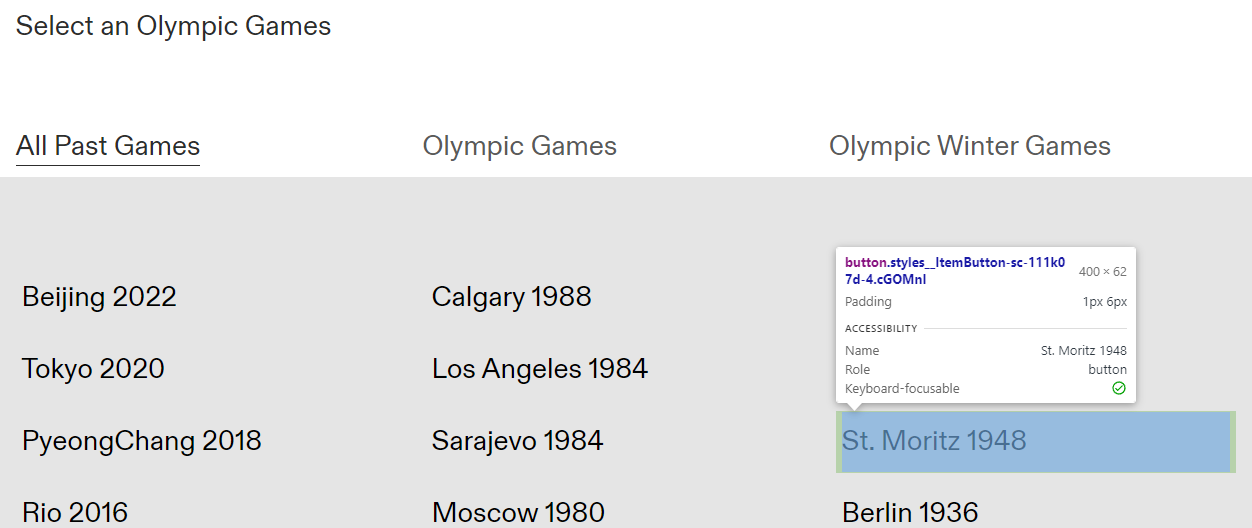
\includegraphics[width=0.87\linewidth]{games-list.png}
    \caption{Widok aplikacji przed wybraniem konkretnych igrzysk}
\end{figure}

\begin{figure}[h!t]
    \centering
    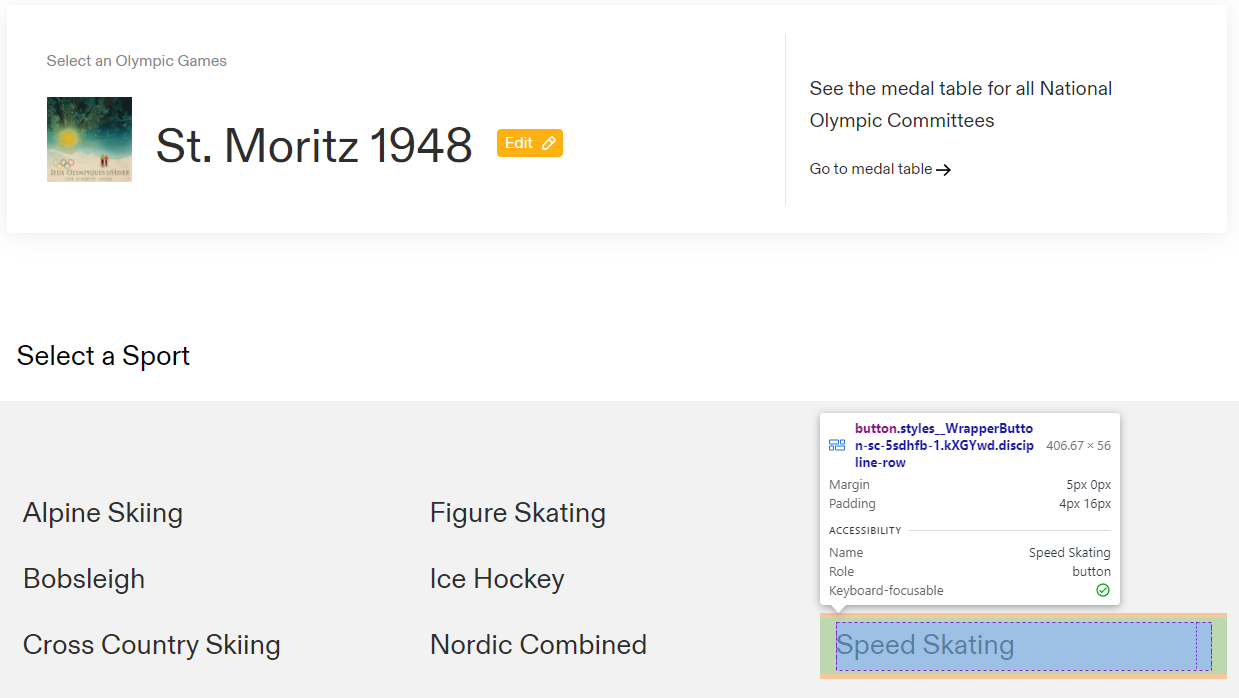
\includegraphics[width=0.87\linewidth]{sport-list.png}
    \caption{Lista sportów po wybraniu konkretnych igrzysk}
\end{figure}

\begin{figure}[h!t]
    \centering
    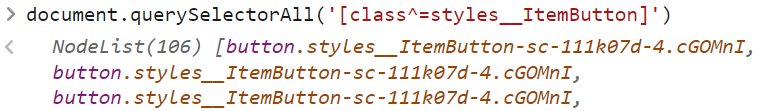
\includegraphics[width=0.5\linewidth]{selector-on-games-list.png}
    \caption{Lista elemntów poszczególnych IO przed interakcją}
\end{figure}

\begin{figure}[h!t]
    \centering
    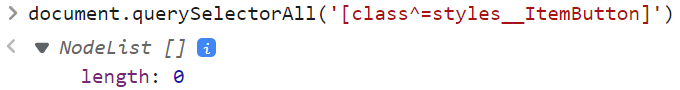
\includegraphics[width=0.5\linewidth]{selector-on-sports-list.png}
    \caption{Lista elemntów poszczególnych IO po interakcji}
\end{figure}

Guziki w poszczególnych listach aplikacji na szczęście są elementami innych klas,
zatem po każdej interakcji wywoływane jest API observera, który czeka na załadowanie
się oczekiwanej klasy guzików i dopiero wtedy kontynuowane jest scrapowanie.
Puppeteer także posiada metodę obiektu strony \verb|waitForSelector|, natomiast 
w naszym zastosowaniu czekanie odbywa się w środowisku przeglądarki, a nie w Node,
zatem niemożliwym było skorzystanie z owej metody.

\subsection{Skrypty ewaluacyjne}
Największą niedogodnością okazało się usuwanie elementów przez aplikację po każdej
interakcji, zamiast np. chowania ich. W związku z tym, niemożliwe było tworzenie
handlerów elementów za pomocą metody \verb|evaluateHandle| i obsługiwanie ich z
poziomu Node'a. Zamiast tego, całą logikę obsługi aplikacji trzeba było wstrzyknąć 
do zawartości strony jako skrypt ewaluacyjny. Z tego samego powodu koniecznym było
wywoływanie metody \verb|querySelectorAll| przy każdym przejściu przez drzewo dyscyplin,
gdyż elementy pobrane w poprzednim przejściu nie istniały już na stronie w trakcie
następnego.

\section{Postępy}
\subsection{Zbiór linków z danymi z poszczególnych dyscyplin sportowych}
Po wykonaniu wyżej opisango scrapowania otrzymano zbiór wszystkich statycznych
stron z wynikami poszczególnych dyscyplin, zapisany jako plik CSV. W poniższej 
tabeli zaprezntowano pierwsze 20 linijek tego pliku (z 6575).
\begin{center}
    \csvautotabular{linkshead20.csv}
\end{center}

Każda z tych stron zawiera zbiór divów klasy \verb|styles__Row-*|. W nim z kolei
dane, które chcemy uzyskać zapisane są w przedstawiony niżej sposób. Scrapowanie
zatem powinno pójść bezproblemowo.
\begin{figure}[ht]
    \centering
    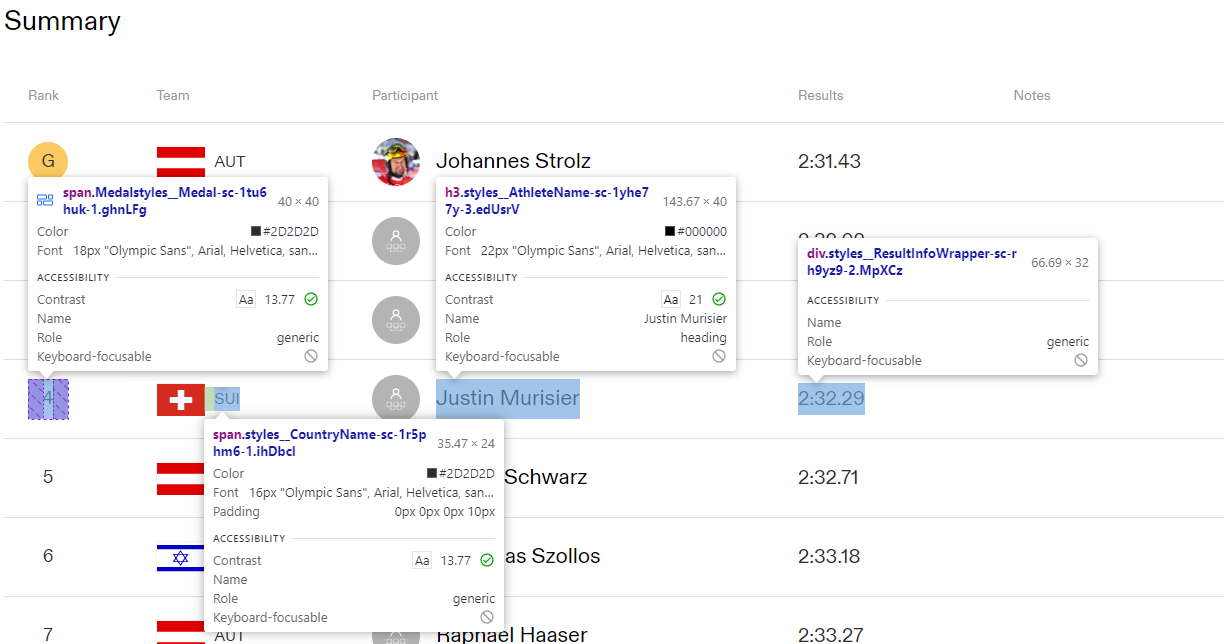
\includegraphics[width=0.8\linewidth]{data-classes.png}
    \caption{klasy poszczególnych danych}
\end{figure}

\end{document}